% DIAPOSITIVA 7: Bolivia -- diseño
\begin{frame}{Etapa 1: Bolivia -- replicación del SOMEN-DC}
  \textbf{Elección seleccionada}
  \begin{itemize}
    \item Bolivia, 2.ª vuelta presidencial, 19 oct.\ 2025
    \item Rodrigo Paz Pereira vs.\ Jorge ``Tuto'' Quiroga
    \item Elección bipolar, no tratada previamente por SOMEN-DC
  \end{itemize}
  \vspace{0.4em}
  \textbf{Dataset}
  \begin{itemize}
    \item \num{153} días de campaña (18 may.\ al 18 oct.\ 2025)
    \item Plataformas: Facebook, Instagram, TikTok, Twitter/X
    \item \num{308} observaciones, \num{26} características
    \item Variable objetivo: interpolación de \num{14} encuestas
          anclada al resultado real: Paz \num{54,53\%}, Quiroga \num{45,47\%}
  \end{itemize}
  \vspace{0.4em}
  \textbf{Modelos entrenados:} 6 especificaciones
  (lineal, lineal más PCA, MLP-BP, MLP-BP más PCA, GRNN)
\end{frame}

% DIAPOSITIVA 8: Bolivia -- gráfica serie de tiempo
\makered
\begin{frame}{Etapa 1: Bolivia -- evolución de la predicción}
  \begin{center}
    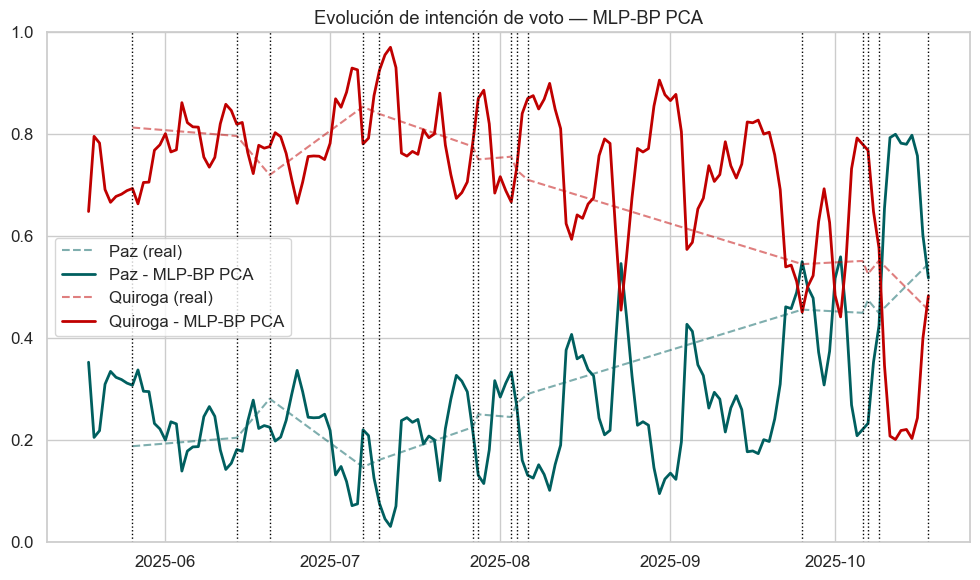
\includegraphics[width=0.88\textwidth]{img/mlp_bp_pca_timeseries.png}
  \end{center}
  {\footnotesize\color{subtleGray}\centering
    Evolución predicha vs.\ encuestas -- MLP-BP+PCA (modelo ganador)}
\end{frame}
\makeblue

% DIAPOSITIVA 9: Bolivia -- resultados
\begin{frame}{Etapa 1: Bolivia -- resultados (día de la elección)}
  \vspace{-0.1em}
  \begin{center}
  \small
  \rowcolors{2}{tableBand}{white}
  \begin{tabular}{L{4.2cm} C{2.0cm} C{1.6cm} C{1.6cm}}
    \toprule
    \rowcolor{barBlue}
    {\color{white}\textbf{Modelo}} &
    {\color{white}\textbf{Pred.\ Paz}} &
    {\color{white}\textbf{MAE}} &
    {\color{white}\textbf{MAPE}} \\
    \midrule
    Baseline (última encuesta) & 36,50\% & 0,1803 & 33,1\% \\
    Regresión lineal           & 24,85\% & 0,2968 & 54,4\% \\
    Regresión lineal + PCA     & 23,38\% & 0,3115 & 57,1\% \\
    MLP-BP                     & 46,91\% & 0,0762 & 14,0\% \\
    \rowcolor{tableBand}
    \textbf{MLP-BP + PCA}      & \textbf{51,74\%} & \textbf{0,0279} & \textbf{5,1\%} \\
    GRNN                       & 34,67\% & 0,1986 & 36,4\% \\
    \midrule
    Resultado real             & \num{54,53\%} & {-} & {-} \\
    \bottomrule
  \end{tabular}
  \end{center}

  \vspace{0.2em}
  \begin{columns}[T]
    \begin{column}{0.55\textwidth}
      \small
      \textbf{Observación metodológica:} MAE y RMSE son idénticos porque $n=1$
      (un solo punto de evaluación). Se reporta MAE y MAPE; la tabla eliminó
      la columna RMSE redundante. [\corr{Corrección 1.9}]
    \end{column}
    \begin{column}{0.41\textwidth}
      \begin{block}{\textbf{PM1}: Respondida}
        \small La replicación es posible.\\
        MLP-BP+PCA supera 6 veces al baseline.
      \end{block}
    \end{column}
  \end{columns}
\end{frame}

% DIAPOSITIVA 10: Bolivia -- limitaciones, PM2
\begin{frame}{Etapa 1: Bolivia -- confirmación de las tres limitaciones}
  \begin{columns}[T]
    \begin{column}{0.52\textwidth}
      \textbf{Las tres limitaciones se verificaron empíricamente:}
      \begin{itemize}
        \item \alrt{No transferibilidad confirmada:}\\
              Los pesos del MLP-BP son específicos de Bolivia.\\
              No existe mecanismo para exportarlos a Colombia.
        \vspace{0.3em}
        \item \alrt{Rezago estructural:}\\
              En la última semana Paz remontó en encuestas.\\
              El modelo, con interacciones acumuladas, no lo capturó.
        \vspace{0.3em}
        \item \alrt{Disociación TikTok:}\\
              Picos de TikTok inyectaban varianza espuria\\
              cuando la intención de voto estaba estacionaria.
      \end{itemize}
    \end{column}
    \begin{column}{0.44\textwidth}
      \begin{alertblock}{\textbf{PM2}: Respondida}
        El paradigma \textit{During-Campaign} no escala:\\
        requiere infraestructura desde el día 1 y\\
        produce pesos no exportables.\\[0.4em]
        \textbf{Conclusión:} necesitamos un enfoque\\
        \textit{fuera de campaña} y agnóstico a la elección.
      \end{alertblock}
      \vspace{0.4em}
      \small
      \textbf{Siguiente paso:} resolver el problema del histórico.
      ¿Cómo conocer el estado de las interacciones en el pasado sin
      haber recolectado datos en tiempo real?
    \end{column}
  \end{columns}
\end{frame}
